% !TEX program = xelatex
% !TEX encoding = UTF-8 Unicode
% !Mode:: "TeX:UTF-8"

\documentclass{resume}
\usepackage{graphicx}
\usepackage{tabu}
\usepackage{multirow}
\usepackage{progressbar}
\usepackage{zh_CN-Adobefonts_external} % Simplified Chinese Support using external fonts (./fonts/zh_CN-Adobe/)
%\usepackage{zh_CN-Adobefonts_internal} % Simplified Chinese Support using system fonts
\usepackage{linespacing_fix} % disable extra space before next section
\usepackage{cite}

\begin{document}
\pagenumbering{gobble} % suppress displaying page number

\Large{
  \begin{tabu}{ c l r }
   \multirow{5}{1in}{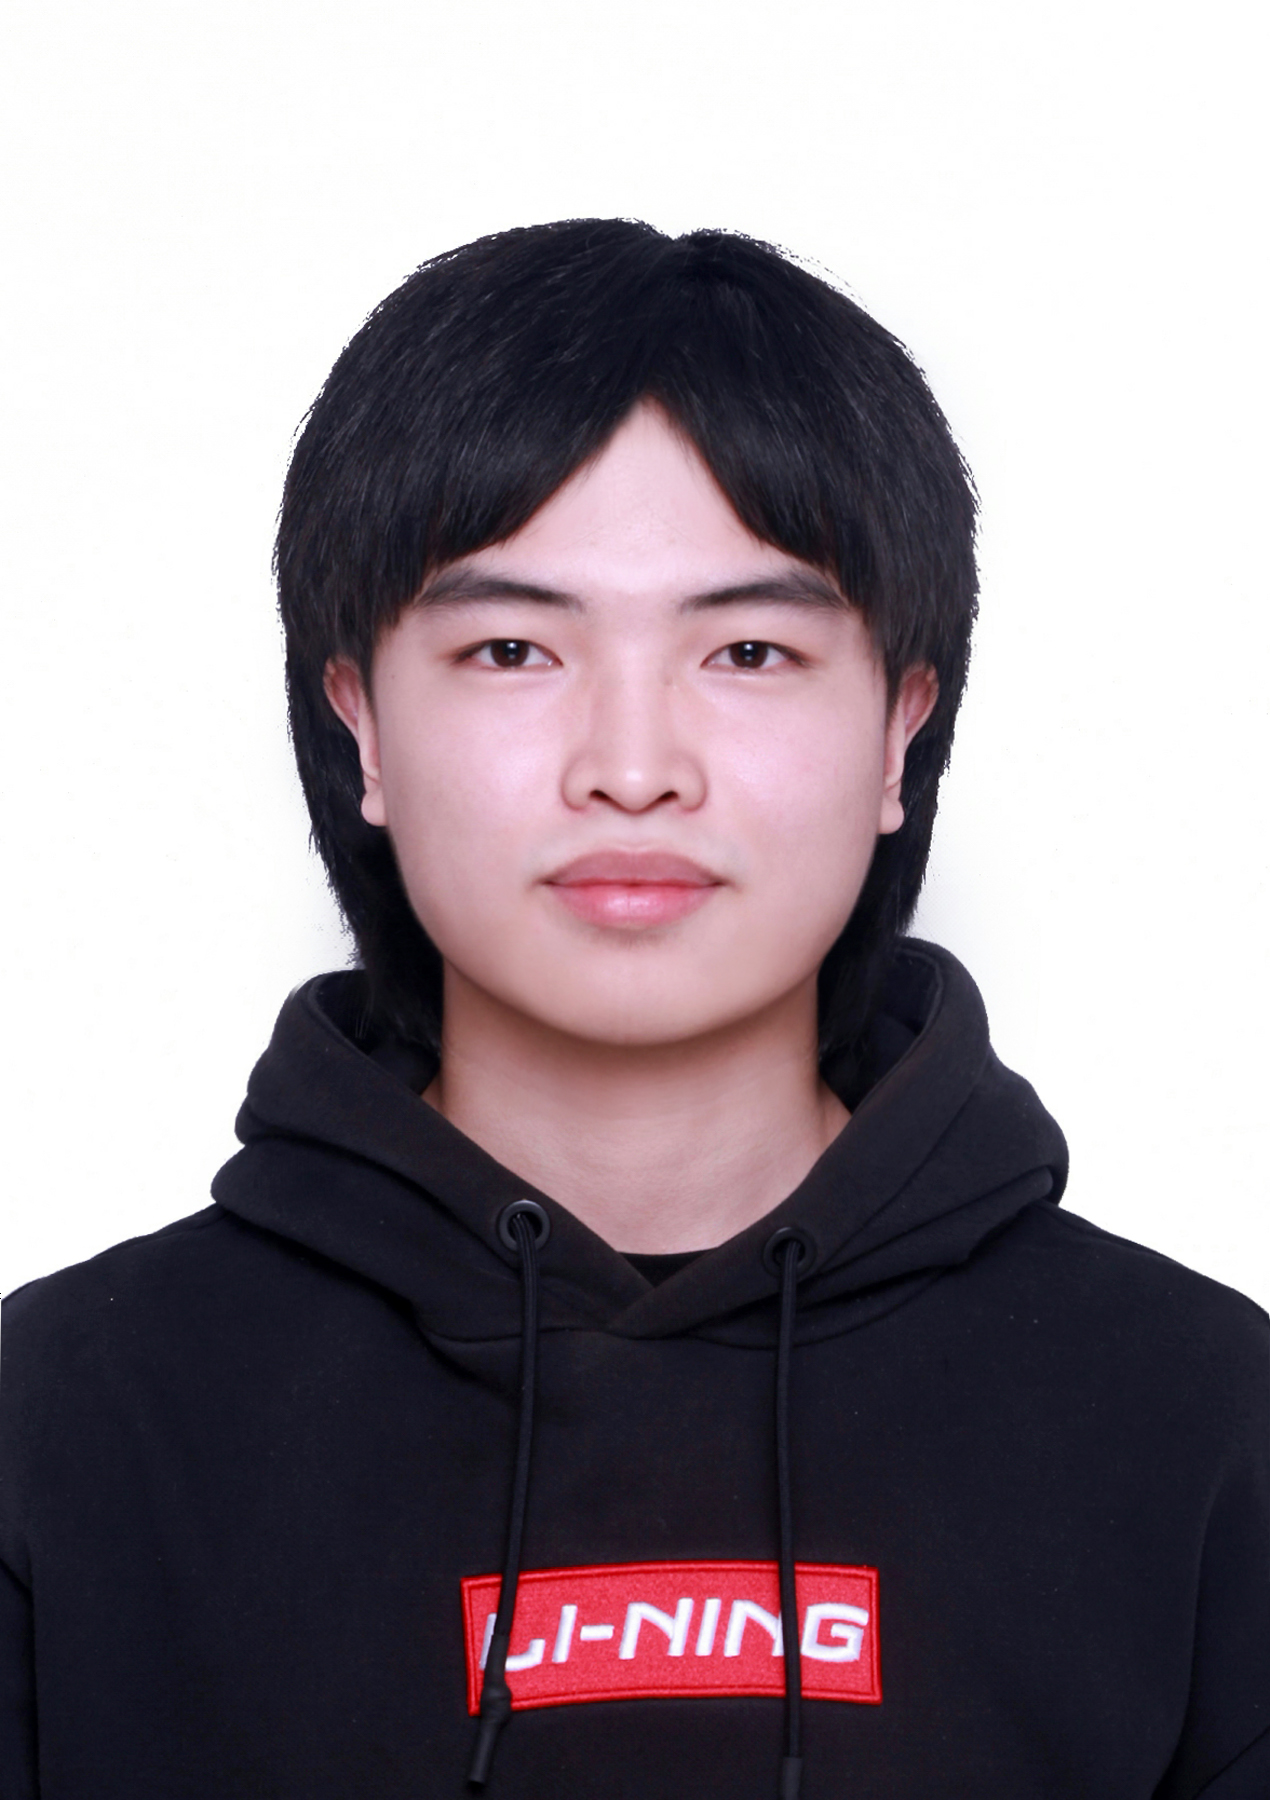
\includegraphics[width=0.88in]{avatar}} & \scshape{段启阳}  \\
    & \email{kiyanda@163.com} & {C~}\progressbar{0.7} \\
    & \phone{(+86) 180-5379-7262} & {C++~}\progressbar{0.7} \\
    & \faWechat {DQY\_78514196} & {Java~}\progressbar{0.6} \\
    & \github[github.com/Kiyanda]{https://github.com/Kiyanda} & {SQL~}\progressbar{0.6} \\
    & \faHome 陕西·汉中 & {Python~}\progressbar{0.6} \\
    & \faHeart Linux开发 & {Shell~}\progressbar{0.6}
  \end{tabu}
}

\normalsize{%字体大小

\section{\faGraduationCap\ 教育背景}
\datedsubsection{\textbf{西北大学},陕西,西安}{2019年9月 -- 至今}
\textit{在读本科生}\ 计算机科学与技术, 预计 2023 年 6 月毕业

\section{\faHeartO\ 获奖情况}
\datedline{\textit{第十三届全国大学生网络安全信息安全竞赛创新实践能力赛西北赛区分区赛}, 三等奖}{2020 年10 月}
\datedline{\textit{第十四届全国大学生网络安全信息安全竞赛创新实践能力赛西北赛区分区赛}, 二等奖}{2021 年10 月}

\section{\faUsers\ 项目经历}
% increase linespacing [parsep=0.5ex]
\datedsubsection{\textbf{哈工大HIT-Linux-0.11 oslab实验} }{2022年9月 }
\role{汇编语言,C语言  }{Linux0.11操作系统}
项目地址:https://github.com/Kiyanda/HIT-Linux-0.11以及书籍《linux-0.11内核完全注释》赵烔·著。
这是网易云课堂选的操作系统所要求的实验的代码及相关记录,授课老师是哈工大的李治军老师,在做实验的过程中阅读了《linux-0.11内核完全注释》这本书,
对初版Linux内核有了一定了解。Linux0.11内核编译的镜像文件在windows wsl2安装的Ubuntu18.04中的bochs虚拟机中运行。
\begin{itemize}
  \item 改写了bootsect.s相关汇编代码,实现了将"DuanOS is booting..."的信息打印在屏幕上,并改变了字体颜色。
  \item 改写了setup.s汇编代码,实现bootsect.s完成setup.s的载入,并跳转到setup.s开始地址执行。而setup.s向屏幕输出一行"Now we are in SETUP"。
  \item 改写了setup.s获取一个基本的硬件参数(内存参数),将其存放在内存的特定地址,并输出到屏幕。
  \item 在Linux 0.11上添加了两个系统调用,并编写了两个简单的应用程序测试它们。
\end{itemize}

\datedsubsection{\textbf{用 Verilog 实现的miniCPU}}{2022年5月 -- 2022年7月}
\role{Verilog, 汇编指令}{计算机体系结构}
使用verilog语言实现微型CPU各模块,并进行组合实现汇编指令集, https://github.com/Kiyanda/miniCPU
\begin{itemize}
  \item 在一定基础上实现了push pop call ret指令,在深层次上理解了栈的工作原理。
  \item 对X86指令集有了一定了解。
\end{itemize}

% Reference Test
%\datedsubsection{\textbf{Paper Title\cite{zaharia2012resilient}}}{May. 2015}
%An xxx optimized for xxx\cite{verma2015large}
%\begin{itemize}
%  \item main contribution
%\end{itemize}


\section{\faCogs\ IT 技能}
% increase linespacing [parsep=0.5ex]
\begin{itemize}[parsep=0.5ex]
  \item 掌握计算机网络,操作系统的基础知识,熟悉常用的数据结构和算法。
  \item 了解linux内核,掌握Linux基础知识,熟悉基本shell指令。会使用版本控制工具Git。
  \item 有云服务器部署经验,熟悉Ubuntu等Linux操作系统。有MySQL、Redis数据库使用经验。
  \item 有Docker使用经验,熟悉Docker工作部署流程。会使用Nginx,有个人网站部署经验。
\end{itemize}


\section{\faInfo\ 其他}
% increase linespacing [parsep=0.5ex]
\begin{itemize}[parsep=0.5ex]
  \item 语言: 英语 - CET4
\end{itemize}

}
%% Reference
%\newpage
%\bibliographystyle{IEEETran}
%\bibliography{mycite}
\end{document}
